\documentclass[12pt]{article}
\usepackage[czech]{babel}
\usepackage[utf8]{inputenc}
\usepackage[plainpages=false,pdfpagelabels,unicode]{hyperref}
\usepackage[pdftex]{graphicx}
\usepackage[margin=2cm, includefoot]{geometry}
\usepackage{wrapfig}

\begin{document}

\title{Praktikum z patologické fyziologie \\
Model venózní trombózy u laboratorního potkana}
\author{Marie Ostrá}
\maketitle

\section{Úvod}

\begin{wrapfigure}{r}{0.4\linewidth}
  \vspace{-20pt}
  \begin{center}
	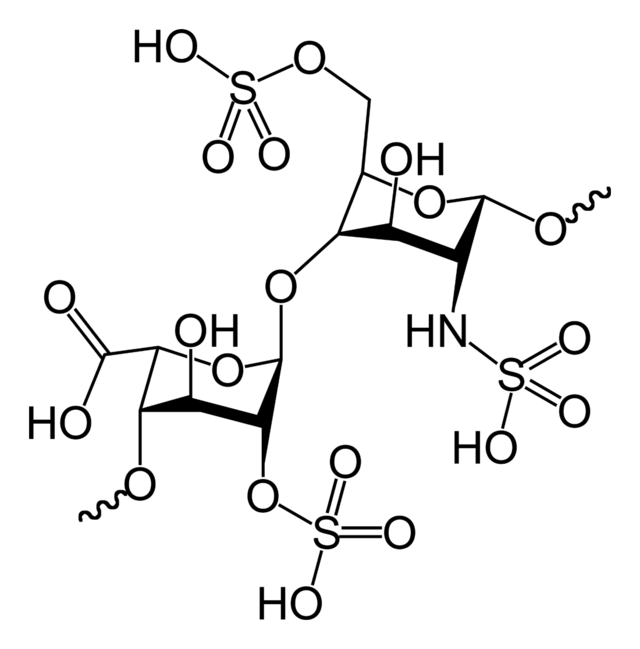
\includegraphics[width=\linewidth]{heparin.png}
	\caption{Heparin}
  \end{center}
  \vspace{-20pt}
\end{wrapfigure}

Trombózou rozumíme vytváření krevních sraženin uvnitř cirkulačního systému. Ke vzniku tohoto
stavu vede poškození cévní stěny (zánětem, aterosklerózou), vyšší srážlivost krve (při poruše
antikoagulačních faktorů nebo uvolněním koagulačních faktorů z poškozené tkáně) a snížená
rychlost průtoku krve (např. u ležících pacientů). K těmto mechanismům přispívá i zvýšená
viskozita krve (u polycytémie, dehydratace apod.).

Mezi přirozené antikoagulační faktory patří specifický endotelový protein trombomodulin a
plazmatické proteiny jaterního původu (protein C, protein S a antitrombin III). Heparin (ať už
tělu vlastní nebo dodávaný za léčebným účinkem) snižuje srážení krve aktivací antitrombinu III.


\section{Postup}
Model venózní trombózy u laboratorního potkana dle Hladovce (1986) umožňuje kvalifikovat i
kvantifikovat tvorbu trombu ve venózním řečišti, která se dá standardně vyvolat společným
působením dvou základních patogenetických mechanismů poškozujících cévní endotel –
působením hypotonického roztoku a stagnací krve ve venózním řečišti. Hmotnost trombu je
možno modifikovat aplikací heparinu. Aktuální situaci v koagulaci je možno monitorovat pomocí
koagulačních testů, např. aPTT (aktivovaný parciální tromboplastinový čas) a TT (trombinový
čas), nebo stanovením koncentrace fibrinogenu.
\subsection{Operační výkon}
Laboratorní potkany po úvodní inhalační anestézii uvedeme do celkové narkózy a 
experimentální zvířata rozdělíme na dvě skupiny:
\begin{itemize}
	\item{1. skupina: experimentální venózní trombóza bez antikoagulační terapie}
	\item{2. skupina: experimentální venózní trombóza s antikoagulační terapií}
\end{itemize}
Zvířatům podáme do vena jugularis 2 ml hypotonického roztoku (25\% roztok fyziologického
roztoku). Ve skupině s antikoagulační terapií přidáme do tohoto roztoku ještě vypočtené
množství heparinu tak, aby zvíře dostalo antikoagulační dávku 4\,U/kg. Zvíře fixujeme na
operačním stolku v poloze na hřbetě. Nůžkami rozstřihneme kraniokaudálně kůži cca 1\,cm
laterálně od manubrium sterni tak, aby byla viditelná v. jugularis externa v místě, kde se zanořuje
pod m. pectoralis. Cévu nepreparujeme! Jehlu zavedeme kraniálně přes m. pectoralis do v.
jugularis tak, aby hrot jehly při jejím mírném zvednutí lehce prosvítal tenkou stěnou žíly. Do
vény velmi pomalu aplikujeme fyziologický roztok (bez nebo s heparinem, podle skupiny).
Operační ránu uzavřeme v jedné vrstvě několika stehy.

Ze střední laparotomie pomocí očního rozvěrače otevřeme dutinu břišní a tupou preparací opatrně
uvolníme cévní svazek abdominální aorty a vena cava inf. tak, aby bylo pod uvolněný cca 2\,cm
dlouhý segment možno naložit dvě ligatury (horní ligatura pod levou renální vénou, dolní cca 2
cm pod horní). Obě ligatury zatáhneme. Po uplynutí 10\,min rozstřihneme hrudník ve stření čáře a
provedeme intrakardiální odběr krve do stříkačky s připraveným citrátem (1:9). Dobře
promíchanou krev ze stříkačky opatrně stříkneme do plastikové zkumavky pro centrifugaci. Po
10\,min centrifugace (3000\,ot) získáme plasmu, kterou dále analyzujeme.

Po odběru krve ze srdce (zvíře uhyne) vystřihneme cévní segment z dutiny břišní a umístíme ho
do vlhké komůrky. Segment zvážíme nejprve celý, pak jej rozstřihneme, opláchneme
fyziologickým roztokem, vysušíme a znovu zvážíme. Z rozdílu obou hmotností vypočítáme
hmotnost trombu (tímto postupem se do jisté míry relativizuje rozdíl v délkách segmentů
izolovaných na jednotlivých pracovištích).

\subsection{Laboratorní část}
\subsubsection{aPTT (aktivovaný parciální tromboplastinový čas)}
Do 0,1 ml plasmy přidáme 0,1 ml kefalinkaolinového reagens a stejné množství 0,025 mol/l
CaCl$_2$. Kefalinová složka reagens aktivuje XII. Hagemannův faktor vnitřní koagulační kaskády.
Kaolinová zrna standardně imitují membrány krevních destiček, které byly od plasmy odděleny
centrifugací. Koagulační faktory obsažené ve vzorku plasmy po aktivaci kefalinkaolinovým
reagens a po přidání 0,025 mol/l CaCl$_2$ začnou srážet fibrinogen v plasmě na fibrin. Dobu srážení
(s) registruje koagulometr jako aPTT.???

\section{Výsledky}

\begin{table}[h!]
\begin{tabular}{|c|c|c|c|c|c|c|c|c|c|}
\hline
Rank Sum & Rank Sum & $U$ & $Z$ & $p$-value & $Z$ & $p$-value & Valid $N$ & Valid $N$ & 2*1sided \\
kontrola & heparin & & & & adjusted & & kontrola & heparin & exact $p$ \\
\hline
3351,5 & 1304,5 & 79,5 & 7,857 & 0,000 & 7,910 & 0,000 & 47 & 49 & 0,000 \\
\hline
\end{tabular}
\caption{Mann-Whitney $U$ Test pro hmotnost trombu. Marked tests are significant at $p < 0,05$}
\end{table}

\begin{table}[h!]
\begin{tabular}{|c|c|c|c|c|c|c|c|c|}
\hline
Max Neg & Max Pos & $p$-level & Mean & Mean & Std.Dev. & Std.Dev. & Valid $N$ & Valid $N$ \\
Differnc & Differnc & & kontrola & heparin & kontrola & heparin & kontrola & heparin \\
\hline
0,00 & 0,875814 & $p <$ .001 & 0,038085 & 0,004306 & 0,031217 & 0,009279 & 47 & 49 \\
\hline
\end{tabular}
\caption{Kolmogorovův-Smirnovův Test pro hmotnost trombu. Marked tests are significant at $p < 0,05$}
\end{table}



\begin{figure}[h!]
	\begin{centering}
	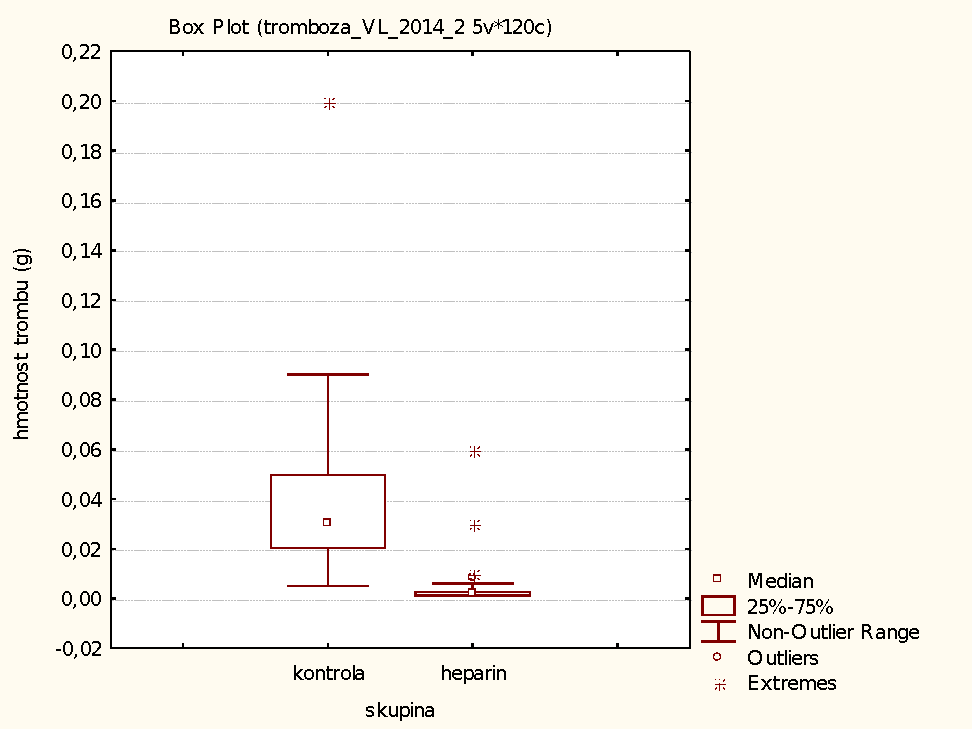
\includegraphics[width=0.7\linewidth]{hmotnost-trombu-box.pdf}
	\caption{Hmotnost trombu}
	\end{centering}
\end{figure}

\begin{figure}[h!]
	\begin{centering}
	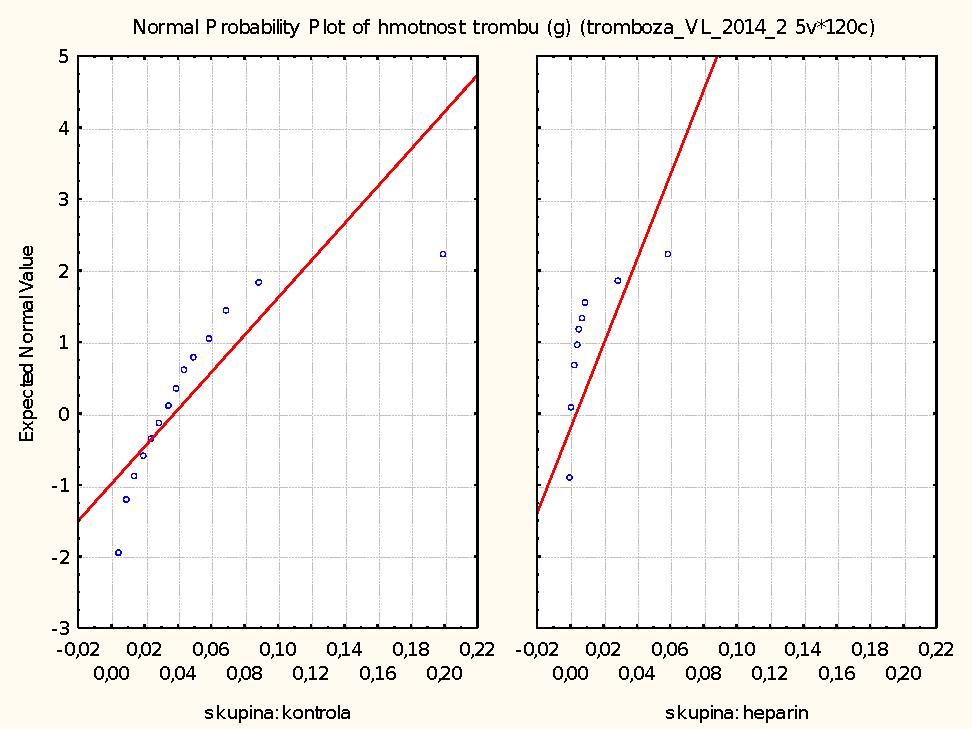
\includegraphics[width=0.7\linewidth]{hmotnost-trombu-prob.pdf}
	\caption{Hmotnost trombu}
	\end{centering}
\end{figure}

\begin{figure}[h!]
	\begin{centering}
	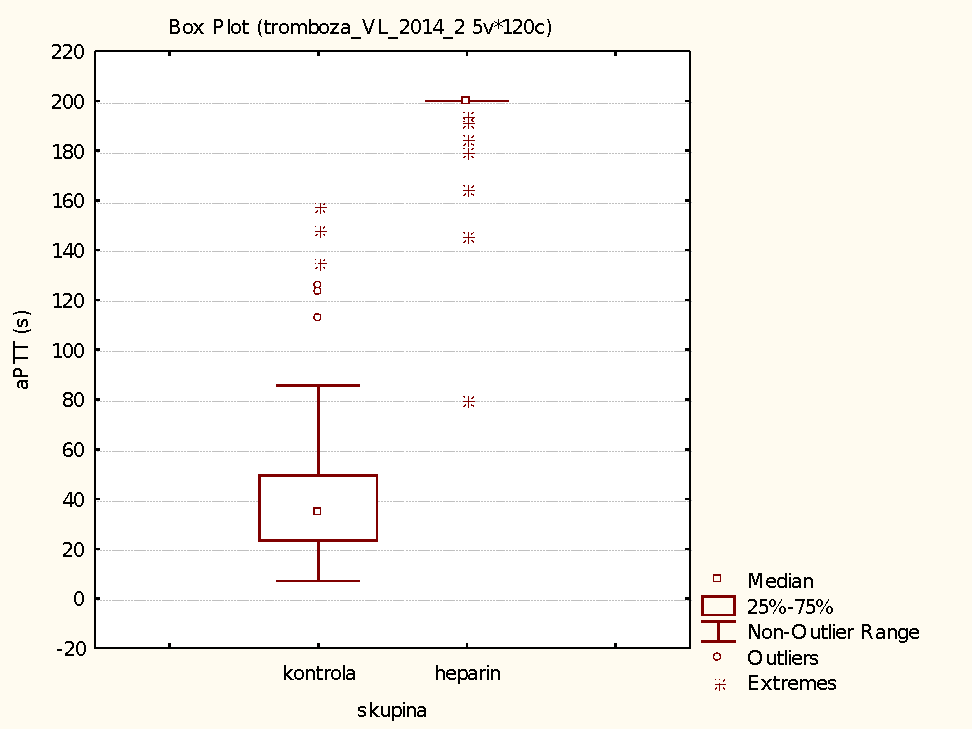
\includegraphics[width=0.7\linewidth]{aPTT-box.pdf}
	\caption{aPTT statistika měřených hodnot}
	\end{centering}
\end{figure}

\begin{figure}[h!]
	\begin{centering}
	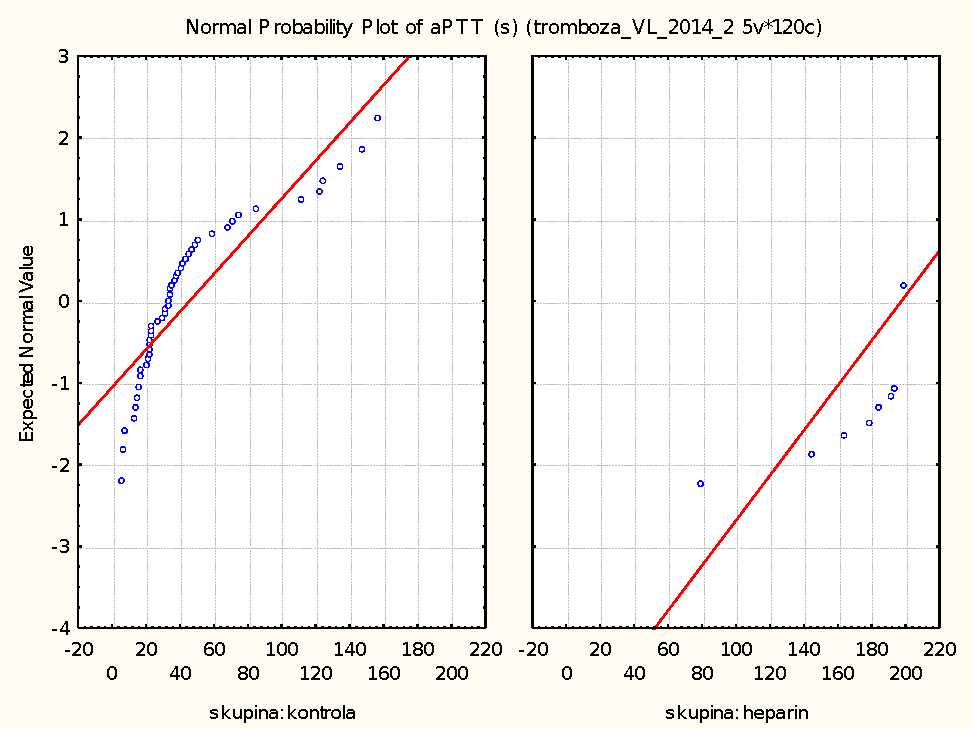
\includegraphics[width=0.7\linewidth]{aPTT-prob.pdf}
	\caption{aPTT porovnání s normálním rozdělením}
	\end{centering}
\end{figure}

\begin{figure}[h!]
	\begin{centering}
	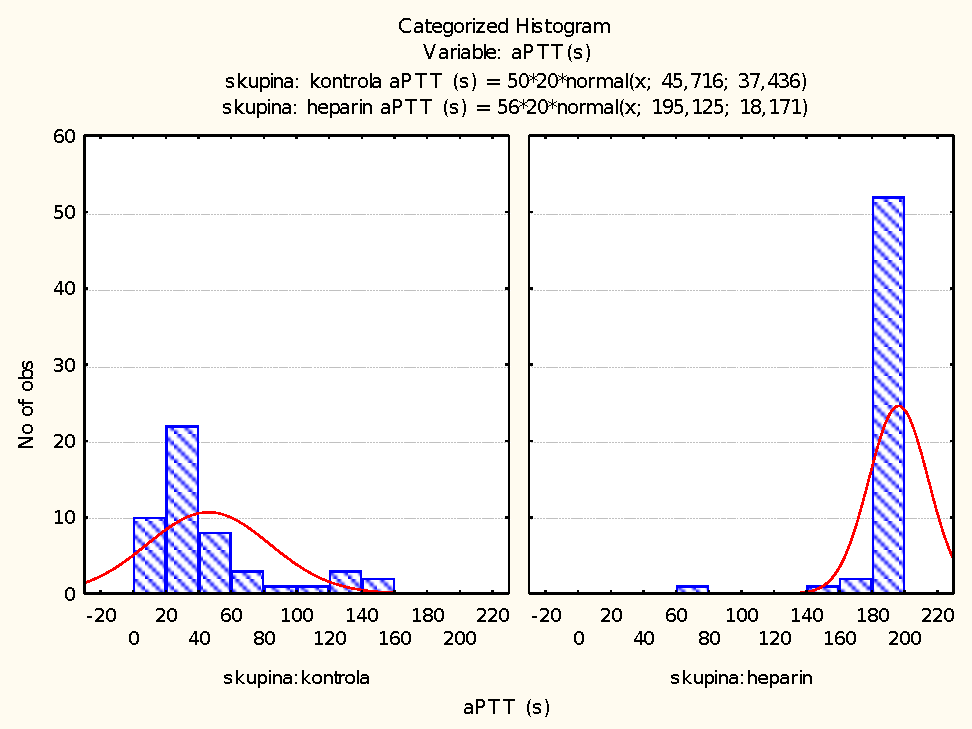
\includegraphics[width=0.7\linewidth]{aPTT-hist.pdf}
	\caption{aPTT histogram}
	\end{centering}
\end{figure}

\begin{table}[h!]
\begin{tabular}{|c|c|c|c|c|c|c|c|c|c|c|}
\hline
Rank Sum & Rank Sum & $U$ & $Z$ & $p$-value & $Z$ & $p$-value & Valid $N$ & Valid $N$ & 2*1sided \\
kontrola & heparin & & & & adjusted & & kontrola & heparin & exact $p$ \\
\hline
1284 & 4387 & -9,243 & 0,000 & 50 & 9,000 & -8,803 & 0,000 & 56 & 0,000 \\
\hline
\end{tabular}
\caption{Mann-Whitney $U$ Test pro aPPT. Marked tests are significant at $p < 0,05$}
\end{table}

\begin{table}[h!]
\begin{tabular}{|c|c|c|c|c|c|c|c|c|}
\hline
Max Neg & Max Pos & $p$-level & Mean & Mean & Std.Dev. & Std.Dev. & Valid $N$ & Valid $N$ \\
Differnc & Differnc & & kontrola & heparin & kontrola & heparin & kontrola & heparin \\
\hline
-0,964286 & 0,00 & $p <$ .001 & 45,71600 & 195,1250 & 37,43604 & 18,17097 & 50 & 56 \\
\hline
\end{tabular}
\caption{Kolmogorovův-Smirnovův Test pro aPTT. Marked tests are significant at $p < 0,05$}
\end{table}

\clearpage

\section{Závěr}
Praktikum proběhlo úspěšně. Pozotrovaná hmotnost trombu u zvířat, kterým byl podán heparin, byla průměrně téměř devětkrát menší než u kontrolních zvířat. Naopak aktivovaný parciální tromboplastinový čas byl u zvířat, kterým byl podán heparin, přibližně čtyřikrát větší než u kontrolních zvířat. Tyto pozorování potvrzují očekávání o vlivu heparinu na krevní srážlivost.

\end{document}
